% This is samplepaper.tex, a sample chapter demonstrating the
% LLNCS macro package for Springer Computer Science proceedings;
% Version 2.20 of 2017/10/04
%
\documentclass[runningheads]{llncs}
%
\usepackage{graphicx}
\usepackage{multirow} 
\usepackage{fancyvrb}
\usepackage[misc,geometry]{ifsym} 


% Used for displaying a sample figure. If possible, figure files should
% be included in EPS format.
%
% If you use the hyperref package, please uncomment the following line
% to display URLs in blue roman font according to Springer's eBook style:
% \renewcommand\UrlFont{\color{blue}\rmfamily}

\begin{document}
%
\title{On Secondary Structure Analysis by Using Formal Grammars and Artificial Neural Networks\thanks{Supported by the Russian Science Foundation grant 18-11-00100}}
%
\titlerunning{Formal Grammars \& Neural Networks}
% If the paper title is too long for the running head, you can set
% an abbreviated paper title here
%
\author{Polina Lunina\inst{1,2}\orcidID{0000-0002-7172-2647} \Letter \and
Semyon Grigorev\inst{1,2}\orcidID{0000-0002-7966-0698}}
%
\authorrunning{Polina Lunina, Semyon Grigorev}
% First names are abbreviated in the running head.
% If there are more than two authors, 'et al.' is used.
%
\institute{Saint Petersburg State University, 7/9 Universitetskaya nab., St. Petersburg, 199034, Russia \and
JetBrains Research, Primorskiy prospekt 68-70, Building 1, St. Petersburg 197374, Russia\\
\email{lunina\_polina@mail.ru \Letter, semyon.grigorev@jetbrains.com, s.v.grigoriev@spbu.ru}\\
}
%
\maketitle              % typeset the header of the contribution
%
\begin{abstract}
A way to combine formal grammars and artificial neural networks for biological sequences processing was recently proposed.
In this approach, an ordinary grammar encodes primitive features of the RNA secondary structure, parsing is utilized for features extraction and artificial neural network~--- for processing of the extracted features.
Parsing is a bottleneck of the solution: input sequences should first be parsed before processing with a trained model which is a time-consuming operation when working with huge biological databases.
In this work, we solve this problem by employing staged learning and limiting parsing to be used only during network training.
We also compare networks which represent the parsing result in two different ways: by a vector and a bitmap image.
Finally, we evaluate our solution on tRNA classification tasks.

\keywords{DNN \and CNN \and Machine Learning \and Secondary Structure \and Genomic Sequences \and Formal Grammars \and Parsing.}
\end{abstract}
%
%
%

\chapter*{Введение}

Теория формальных языков находит применение не только для ставших уже классическими задач синтаксического анализа кода (языков программирования, искусственных языков) и естественных языков, но и в других областях, таких как статический анализ кода, графовые базы данных, биоинформатика, машинное обучение.

Например, в машинном обучении использование формальных грамматик позволяет передать искусственной нейронной сети, предназначенной для генерации цепочек с определёнными свойствами (генеративной нейронной сети), знания о синтаксической структуре этих цепочек, что позволяет существенно упростить процесс обучения и повысить качество результата~\cite{10.5555/3305381.3305582}.
Вместе с этим, развиваются подходы, позволяющие нейронным сетям наоборот извлекать синтаксическую структуру (строить дерево вывода) для входных цепочек~\cite{kasai-etal-2017-tag,kasai-etal-2018-end}.

В биоинформатике формальные грамматики нашли широкое применение для описания особенностей вторичной структуры геномных и белковых последовательностей~\cite{Dyrka2019,WJAnderson2012,zier2013rna}.
Соответствующие алгоритмы синтаксического анализа используются при создании инструментов обработки данных.

Таким образом, теория формальных языков выступает в качестве основы для многих прикладных областей, а алгоритмы синтаксического анлиза применимы не только для обработки естественных языков или языков программирования.
Нас же в данной работе будет интересовать применение теории формальных языков и алгоритмов синтаксического анализа для анализа графовых баз данных и для статического анализа кода.

Одна из классических задач, связанных с анализом графов --- это поиск путей в графе.
Возможны различные формулировки этой задачи.
В некоторых случаях необходимо выяснить, существует ли путь с определёнными свойствами между двумя выбранными вершинами.
В других же ситуациях необходимо найти все пути в графе, удовлетворяющие некоторым свойствам или ограничениям. 
Например, в качестве ограничений можно указать, что искомый путь должен быть простым, кратчайшим, гамильтоновым и так далее.

Один из способов задавать ограничения на пути в графе основан на использовании формальных языков.
Базовое определение языка говорит нам, что язык --- это множество слов над некоторым алфавитом.
Если рассмотреть граф, рёбра которого помечены символами из алфавита, то путь в таком графе будет задавать слово: достаточно соединить последовательно символы, лежащие на рёбрах пути.
Множество же таких путей будет задавать множество слов или язык.
Таким образом, если мы хотим найти некоторое множество путей в графе, то в качестве ограничения можно описать язык, который должно задавать это множество.
Иными словами, задача поиска путей может быть сформулирована следующим образом: необходимо найти такие пути в графе, что слова, получаемые конкатенацей меток их рёбер, принадлежат заданному языку.
Такой класс задач будем называть задачами поиска путей с ограничениям в терминах формальных языков.

Подобный класс задач часто возникает в областях, связанных с анализом граф-структурированных данных и активно исследуется~\cite{doi:10.1137/S0097539798337716,axelsson2011formal,10.1007/978-3-642-22321-1_24,Ward:2010:CRL:1710158.1710234,barrett2007label,doi:10.1137/S0097539798337716}.
Исследуются как классы языков, применяемых для задания ограничений, так и различные постановки задачи.

Граф-структурированные данные встречаются не только в графовых базах данных, но и при статическом анализе кода: по программе можно построить различные графы отображающие её свойства.
Скажем, граф вызовов, граф потока данных и так далее.
Оказывается, что поиск путей в специального вида графах с использованием ограничений в терминах формальных языков позволяет исследовать некоторые свойства программы.
Например проводить межпроцедурный анализ указателей или анализ алиасов~\cite{Zheng,10.1145/2001420.2001440,10.1145/2714064.2660213}, строить срезы программ~\cite{10.1145/193173.195287}, проводить анализ типов~\cite{10.1145/373243.360208}.

В данной работе представлен ряд алгоритмов для поиска путей с ограничениями в терминах формальных языков.
Основной акцент будет сделан на контекстно-свободных языках, однако будут затронуты и другие классы: регулярные, многокомпонентные контекстно-свободные (Multiple Context-Free Languages, MCFL~\cite{!!!}) и конъюнктивные языки.
Будет показано, что теория формальных языков и алгоритмы синтаксического анализа применимы не только для анализа языков программирования или естественных языков, а также для анализа графовых баз данных и статического анализа кода, что приводит к возникновению новых задач и переосмыслению старых.


Структура данной работы такова.
Сперва, в главе~\ref{chpt:GraphTheoryIntro} мы рассмотрим основные понятия из теории графов, необходимые в данной работе.
Затем, в главе~\ref{chpt:FormalLanguageTheoryIntro} мы введём основные понятия из теории формальных языков.
Далее, в главе~\ref{chpt:CFPQ} рассмотрим различные варианты постановки задачи поиска путей с ограничениями в терминах формальнх языков, обсудим базовые свойства задач, её разрешимость в различных постановках и т.д..
И в итоге зафиксируем постановку, которую будем изучать далее.
После этого, в главах~\ref{chpt:CFPQ_CYK}--\ref{chpt:CFPQ_Derivatives} мы будем подробно рассматривать различные алгоритмы решения этой задачи, попутно вводя специфичные для рассматриваемого алгоритма структуры данных.
Большинство алгоритмов будут основаны на классических алгоритмах синтаксического анализа, таких как CYK или LR.
Все главы, начиная с~\ref{chpt:GraphTheoryIntro}, снабжены списком вопросов и задач для самостоятельного решения и закрепления материала.
\section{Ordinary Context-Free Grammars and Artificial Neural Networks for Secondary Structure Analysis}

In this section we provide a brief description of the approach for genomic sequences secondary structure analysis which is proposed in~\cite{grigorevcomposition}.

The secondary structure of RNA sequences can be viewed as a composition of stems~\cite{MQbioinformatics19}. 
So, one can create an ordinary context-free grammar which describes a set of such compositions and use it to extract the actual features of the given sequence. 
Grammar $G_0$ presented in figure~\ref{gram} is an example of such grammar.
This grammar is used in~\cite{grigorevcomposition} as well as in the present work.
This grammar considers only the conventional base pairs (line \textbf{5}) and describes the recursive composition of stems which are at least three base pairs in height (lines \textbf{7-12}).
Stems may be connected by an arbitrary sequence of length from 2 up to 10, and loops also have length from 2 up to 10 (line \textbf{2}).
These parameters were tuned manually as a result of several experiments and can be changed to provide a better grammar for some specific goal.

\begin{figure}
\begin{Verbatim}[numbers=left,xleftmargin=5mm]
s1: stem<s0>
any_str : any_smb*[2..10]
s0: any_str | any_str stem<s0> s0
any_smb: A | U | C | G
stem1<s>: A s U | G s C | U s A | C s G 
stem2<s>: stem1< stem1<s> >
stem<s>:  
      A stem<s> U 
    | U stem<s> A 
    | C stem<s> G 
    | G stem<s> C 
    | stem1< stem2<s> >  
\end{Verbatim}
\caption{Context-free grammar $G_0$ for RNA secondary structure features description}
\label{gram}
\end{figure}

The result of a parsing algorithm for an input string $w$ and a fixed grammar non-terminal $N$ (start nonterminal) is an upper-triangular boolean matrix $M_N$, where $M_N [i,j] = 1$, iff the substring $w[i,j-1]$ is derivable from $N$.
This means that, for the grammar $G_0$, a matrix contains $1$ in a cell iff a correspondent substring folds to a  stem of height at least 3.
Such stem results in a diagonal chain of one-s in the matrix.
Figure~\ref{fig:example} presents the parsing result for a sequence

\[
w_1 = CCCCATTGCCAAGGACCCCACCTTGGCAATCCC
\]

w.r.t the grammar $G_0$.
Colored boxes map a substring which folds to a stem to correspondent cells in the matrix. 
Besides, this matrix contains other non-zero cells, because parser detects all possible foldings for all possible substrings. 
It can be either noise or some important information about the secondary structure. 
One of the tasks that the neural network should perform is to process such matrices and filter all the insignificant contacts between the nucleotides.

\begin{figure}[h]
\begin{center}
\centering
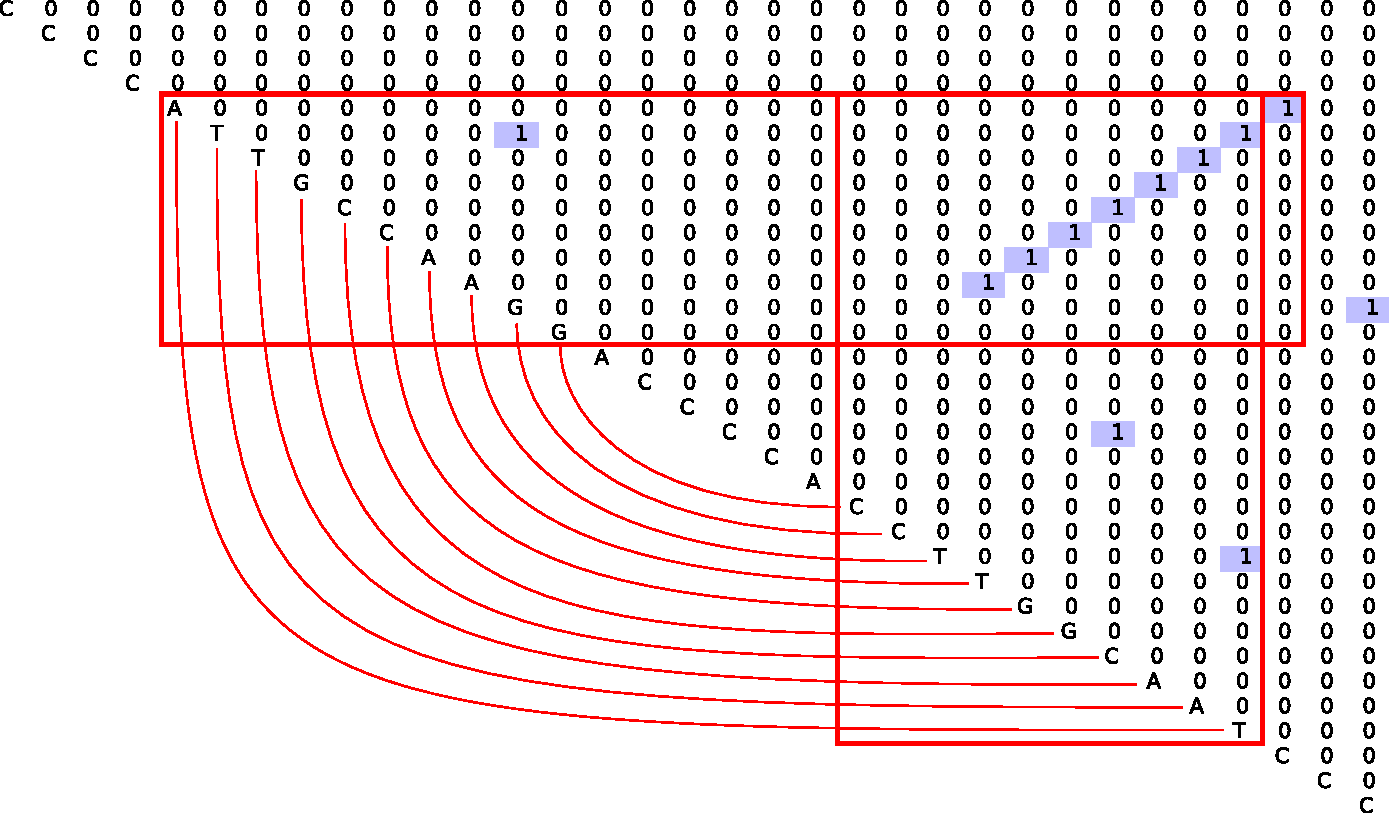
\includegraphics[width=0.8\textwidth]{figures/4.pdf}
\caption{Parsing result for sequence which should fold to
stem}
\label{fig:example}
\end{center}
\end{figure}

The parsing result in a form of a matrix can be linearized, compressed into a byte or integer vector, and be further handled by a dense neural network, as described in~\cite{grigorevcomposition}.
Unfortunately, linearization breaks data locality: a diagonal chain of one-s, which signifies a high stem, is local in a matrix, but is broken apart during its linearization.
We see it to be an argument to investigate the applicability of convolutional networks for parsing result handling, as a boolean matrix can be converted to a black-white bitmap image.
In this paper, we provide an empirical comparison of networks which handle vectors and images.

Another problem is a bad performance of the earlier solution.
Since the trained network handles parsing result, each input sequence should first be parsed.
Parsing is a very time-consuming step: context-free parsing has cubic complexity in terms of the input length.
Even if we use matrix-based parsing algorithm~\cite{Azimov:2018:CPQ:3210259.3210264} which utilizes GPGPU, performance is insufficient.
We believe it would be better to avoid the parsing step at the final stage of the solution.
In this work, we propose a way to solve this problem by building a network which handles raw sequences, not parsing results.

\section{Convolutional Neural Network Utilization}

First, we describe how to use a convolutional network for parsing result processing. Parsing result is a boolean matrix that contains the information about sequence secondary structure features and we utilize the artificial neural network to detect sufficient features and find patterns in their appearance.
Therefore, we need to transform these boolean matrices to some data structure acceptable by the neural network.
Currently, we came up with two possible ways: vectorization and conversion to a black and white image.

The first way is to drop out the nullary bottom left triangle, vectorize the top right triangle row by row and transform it into a byte vector.
This approach reduces the input size, but it requires all the input sequences to have equal length.
Thus we propose to either cut sequences to be of some predefined length or to pad them up with some blank symbols.
Vectorization breaks data locality which makes learning harder: the network should restore back the relations broken during linearization.
This also means that learning takes more time.

The second way is to represent the matrix as an image: the false bits of the matrix as white pixels and the true bits as black ones.
This approach makes it possible to process sequences of different lengths since the images are easily transformed to a specified size.
Data locality is also preserved: the information about relative positions of extracted basic features does not get lost which should improve learning.

The architecture of the neural network that takes vectorized data as an input is described in~\cite{grigorevcomposition} and it consists of the long sequence of interchangeable dense and dropout layers with aggressive batch normalization. 
To handle images, we propose to use a network which consists of a small number of convolutional layers, linearization, and dense network which has a similar architecture as for vectorized data.
An example of the proposed architecture is provided in figure~\ref{nn} (network \textbf{\texttt{N1}}).

\section{Parsing Step Elimination}

Another improvement that we came up with concerns parsing elimination in the context of our solution. 
The idea is to create a model which can handle original sequences instead of the parsing matrices. For that, we propose to use two-staged learning: first, a network which solves a subtask is trained and then it is used as pretrained layers in the training of the resulting network.
In our solution, we first train a neural network to handle parsing results which performs classification according to a problem at hands. We create two networks in order to compare different architectures: one of them handles vectorized parsing result, the other handles parsing result represented as a bitmap image. After that, we extend these neural networks by several input layers that take the initial nucleotide sequence as an input and convert it to the parsing result which is handled appropriately by the pretrained layers.

Figure~\ref{nn} represents the detailed description of these three neural networks architectures.
Here \textbf{\texttt{N1}} is a network which handles images, \textbf{\texttt{N2}} is a network which handles vectorized parsing results, and \textbf{\texttt{N0}} is an additional block which converts the input sequence into a set of features which can be handled by using \textbf{\texttt{N1}} or \textbf{\texttt{N2}}. So, firstly we train \textbf{\texttt{N1}} and \textbf{\texttt{N2}} on parsed data. After that, for vector-based network we combine the extension \textbf{\texttt{N0}} and the whole original sequence of layers and for image-based network we use the similar architecture, except we remove the convolutional layer from the extended model, thus, the first layer at the junction of the blocks corresponds to the linearized image.

\begin{figure}[h]
\begin{center}
\centering
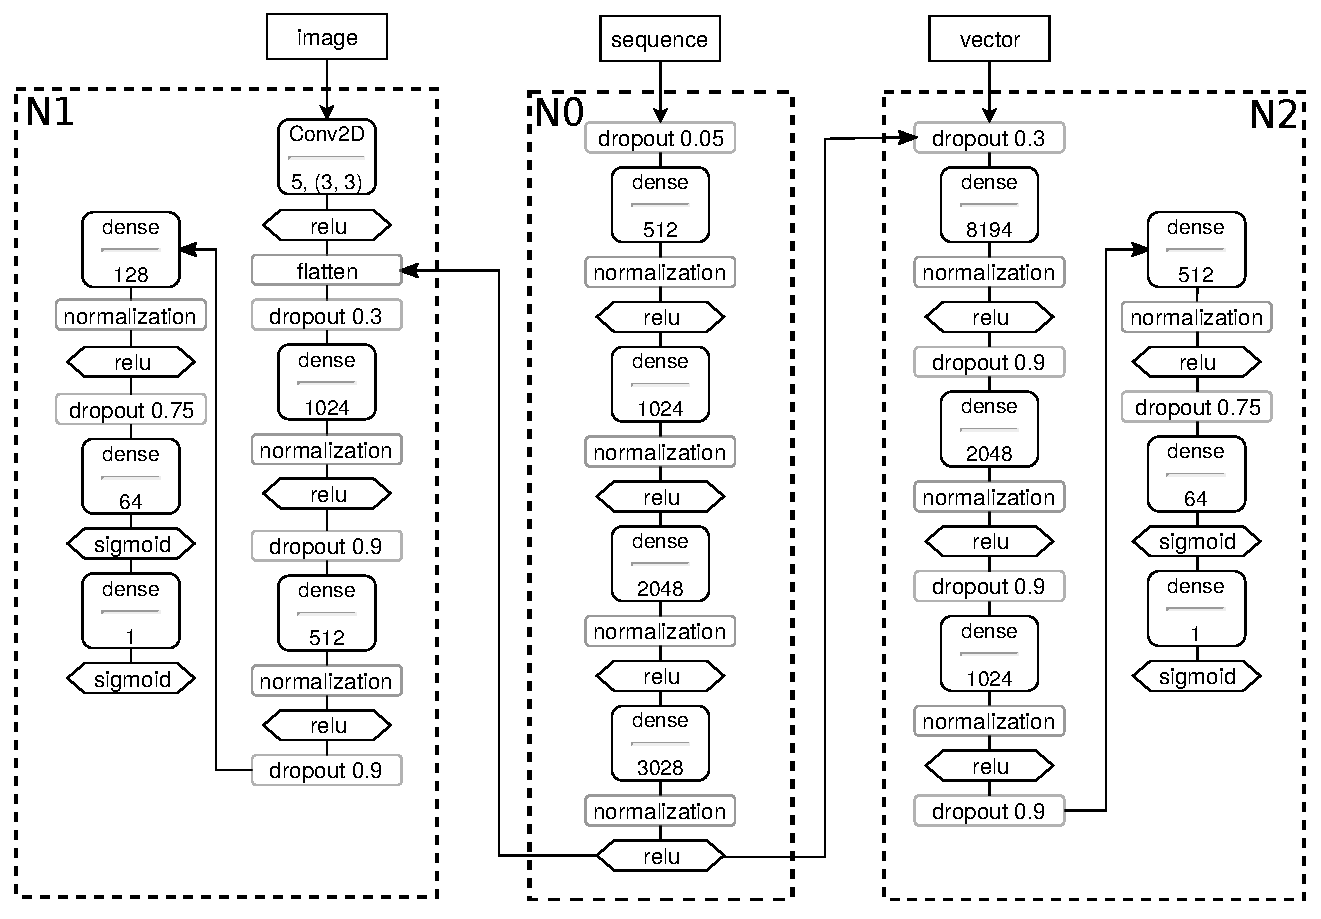
\includegraphics[width=12cm]{figures/nn_arch.pdf}
\caption{Neural networks architectures}
\label{nn}
\end{center}
\end{figure}

To sum up, we developed a technique to process parsing matrices as images by convolutional neural networks. 
Also, we built a model that handles sequences and requires parsing only for training the network it is based on. 
This removes the parsing step from the usage of the trained model.

\section{Evaluation}
We evaluated the proposed approach with the described above modifications on two tRNA sequences analysis tasks.
The first one was a classification of tRNA into two classes: eukaryotes and prokaryotes, while the second was a classification into four classes: archaea, bacteria, plants and fungi.

We used the neural networks shown in the figure~\ref{nn} each of them having the following hyperparameters.
\begin{itemize}
    \item Batch size --- 64.
    \item Cross entropy loss function.
    \item Adagrad optimizer (adaptive gradient) with learning rate 0.05.
\end{itemize}


We took sequences from tRNA databases GtRNAdb\footnote{GtRNAdb tRNA database Web page: \url{http://gtrnadb.ucsc.edu/}. Access date: 05.06.2019.}~\cite{chan2016gtrnadb} and tRNADB-CE\footnote{The tRNADB-CE tRNA database Web page: \url{http://trna.ie.niigata-u.ac.jp/cgi-bin/trnadb/index.cgi}. Access date: 05.06.2019.}~\cite{abe2014trnadb} for these experiments.
We used the parsing algorithm implemented by means of the YaccConstructor\footnote{YaccConstructor is an SDK for syntax analysis tools development. Project repository on GitHub: \url{https://github.com/YaccConstructor/YaccConstructor}. Access date: 07.03.2020.} platform and Keras library~\cite{chollet2015keras} with Tensorflow framework~\cite{tensorflow2015-whitepaper} for neural networks training and testing.
All models, as well as parsing tool, were run on GPU NVIDIA GeForce GTX 1070.
We selected the equal number of samples (single tRNA molecule sequences) for each class for both classification tasks.
Each sample was parsed w.r.t. the grammar $G_0$ and then both vectorized and transformed into an image.
After that, we trained two neural networks: the first handles the representation of the parsing result as vectors, and the second~--- as images.
Finally, we trained the extended neural network.
It consists of a block which takes an initial tRNA sequence as an input and transforms it into the parsing result, and the block of pretrained layers: either the vector- or the image-based model from the previous step. 

All extended neural networks were trained, validated (by hold-out validation) and tested on the same datasets as the corresponding base ones.
The trained models for two classes (EP) and for four classes (ABFP) classification tasks were estimated by using classical machine learning metrics: accuracy, precision and recall.

Accuracy metrics for each problem for the test datasets are presented in the table~\ref{acc}, where base model is a model which handles parsing result (image or vector respectively) and extended model handles tRNA sequences and extends the corresponding base model. Also, this table shows the total time spent on two stages of training (base network + extended network) for both problems and types of data.

\begin{table}[h]
\centering
\caption{Base and extended models test results by accuracy metrics}
\begin{tabular}{|l||l|l||l|l|}
\hline
Classifier                                                               & \multicolumn{2}{l||}{EP}               & \multicolumn{2}{l|}{ABFP}           \\ \hline \hline
Approach                                                                 & Vector-based       & Image-based      & Vector-based      & Image-based     \\ \hline
\begin{tabular}[c]{@{}l@{}}Base model\\ accuracy\end{tabular}            & 94.1\%             & 96.2\%           & 86.7\%            & 93.3\%          \\ \hline
\begin{tabular}[c]{@{}l@{}}Extended model \\ accuracy\end{tabular}       & 97.5\%             & 97.8\%           & 96.2\%            & 95.7\%          \\ \hline
\begin{tabular}[c]{@{}l@{}}Total training \\ time\end{tabular}       & 30000s             & 4600s           & 31800s            & 3600s          \\ \hline
\begin{tabular}[c]{@{}l@{}}Samples for\\ train:valid:test\end{tabular} & \multicolumn{2}{l||}{\begin{tabular}[c]{@{}l@{}}20000:5000:10000\\ (57\%:14\%:29\%)\end{tabular}} & \multicolumn{2}{l|}{\begin{tabular}[c]{@{}l@{}}8000:1000:3000\\ (67\%:8\%:25\%)\end{tabular}} \\ \hline
\end{tabular}
\label{acc}
\end{table}


The estimations by precision and recall metrics for extended models for both classifiers on the same samples as in the  table~\ref{acc} are presented in the table~\ref{pe}.

\begin{table}[h]
\centering
\caption{Extended models test results by precision and recall metrics for each class}
\begin{tabular}{|l||l|l|l|l|l|}
\hline
\multirow{2}{*}{Classifier} & \multirow{2}{*}{Class} & \multicolumn{2}{l|}{Vector-based approach} & \multicolumn{2}{l|}{Image-based approach} \\ \cline{3-6} 
                            &                        & precision         & recall        & precision        & recall        \\ \hline \hline
\multirow{2}{*}{EP}         & prokaryotic            & 95.8\%            & 99.4\%        & 96.2\%           & 99.4\%        \\ \cline{2-6} 
                            & eukaryotic             & 99.4\%            & 95.6\%        & 99.4\%           & 99.5\%        \\ \hline \hline
\multirow{4}{*}{ABFP}       & archaeal               & 91.1\%            & 99.2\%        & 91.6\%           & 98.5\%        \\ \cline{2-6} 
                            & bacterial              & 96.6\%            & 95.1\%        & 95.2\%           & 95.5\%        \\ \cline{2-6} 
                            & fungi                  & 98.5\%            & 94.9\%        & 97.5\%           & 94.3\%        \\ \cline{2-6} 
                            & plant                  & 99.4\%            & 95.7\%        & 99.2\%           & 94.7\%        \\ \hline
\end{tabular}
\label{pe}
\end{table}

The results show that our approach is applicable to tRNA classification tasks and both vector- and image-based models can be used along with dense and convolutional layers in neural networks architectures.
While the differences in results for extended models are insignificant, for base models image-based network demonstrates slightly better results (see table~\ref{acc}).
We believe that the reason of this effect lays in a better locality of features in the image-based representation of parsing result: chain of one-s which means a high stem is local in terms of picture but is broken during linearization. 
Also, we analyzed the time spent on all the models training (table~\ref{acc}) and, although some of these numbers could probably be decreased by more detailed networks tuning, we can state that the image-based networks learn much faster than the vector-based ones.
The current model for images classification uses a single convolutional layer.
Whether it is possible to utilize deep convolutional networks for secondary structure analysis in the discussed approach is a question for future research.

The idea of the extended model that handles sequences instead of parsing results is proved to be applicable in practice and it demonstrates even higher quality than the original parsing-based model, as illustrated by table~\ref{acc}.
We can conclude that it is possible to use parsing only for network training without decreasing the network quality.

To demonstrate the advantage of this technique in practical use 
in comparison with the classical way (when sequences should first be parsed) we took 100 tRNA sequences from two classes: eukaryotes and prokaryotes and used all four of the trained models to predict their classes. While using base models each sequence was parsed, transformed to correspondent format (image or vector) and fed to the neural network. Extended networks run on original sequences, so the parsing step was skipped. We measured the total time required to output predicted class for all the considered sequences in each case. In the table~\ref{time} the results of this experiment are provided and it is clear that the time spent for parsing is crucial relative to the total working time. So, parsing elimination significantly improves the performance of our solution.


\begin{table}[]
\centering
\caption{Time measurements for 100 sequences processing}
\begin{tabular}{|p{2cm}||p{2cm}|p{2cm}|p{2cm}|p{2cm}|}
\hline
\multirow{2}{*}{Step} & \multicolumn{2}{l|}{Vector based approach} & \multicolumn{2}{l|}{Image based approach} \\ \cline{2-5} 
 & \begin{tabular}[c]{@{}l@{}}Base \end{tabular} & \begin{tabular}[c]{@{}l@{}}Extended \end{tabular} & \begin{tabular}[c]{@{}l@{}}Base \end{tabular} & \begin{tabular}[c]{@{}l@{}}Extended \end{tabular} \\ \hline \hline
Parsing & 307.6s & --- & 310.5s & --- \\ \hline
Weights loading & 0.2s & 0.2s & 0.1s & 0.3s \\ \hline
Class predicting & 0.2s & 0.2s & 0.2s & 0.3s \\ \hline
Total & 308.0s & 0.4s & 310.8s & 0.6s \\ \hline
\end{tabular}
\label{time}
\end{table}

\section{Conclusion}
We describe the modifications of the proposed approach~\cite{grigorevcomposition} for biological sequences analysis using the combination of formal grammars and neural networks.
We show that it is possible to improve the quality of the solution by representing parsing result as an image and handling it by using convolutional layers while processing it with a neural network.
Also, we provide a technique that removes the parsing step from the trained model use and allows to run models on the original RNA sequences.
As a result, the performance of the solution is significantly improved.
We demonstrate the applicability of the proposed modifications for real-world problems\footnote{
Project description is available at the project page: \url{https://research.jetbrains.org/groups/plt\_lab/projects?project\_id=43}.
Source code and documentation are published at GitHub: \url{https://github.com/LuninaPolina/SecondaryStructureAnalyzer}. Access date: 07.03.2020}.

We can provide several directions for future research.
First of all, it is necessary to investigate the applicability of the proposed approach for other sequences processing tasks such as 16s rRNA processing and chimeric sequences filtration.

Another possible application is a secondary structure prediction.
We plan to investigate the possibility of creating a network which generates the most possible contact map for the given sequence.
It is necessary to compare this approach with both classical approaches and tools for secondary structure prediction~\cite{jabbari2014fast,jabbari2007hfold,sato2009centroidfold,10.1093/bioinformatics/btr215} and artificial neural network-based ones~\cite{Lu2019,Singh2019}.

The image-based model demonstrates a higher quality.
We believe that it is caused by a better locality of features.
If so, it should be possible to create a deep convolutional network for secondary structure analysis: further investigation is needed.

Finally, it is important to find a theoretical base for grammar tuning.
It is important to adopt the theoretical results on secondary structure description by using formal grammar, such as~\cite{MQbioinformatics19} to find the optimal grammar for our approach.



%
% ---- Bibliography ----
%
% BibTeX users should specify bibliography style 'splncs04'.
% References will then be sorted and formatted in the correct style.
%
\bibliographystyle{splncs04}
\bibliography{main}

\end{document}
